\documentclass[addpoints,12pt]{exam}
\usepackage{amsmath}
\usepackage{amsthm}
\usepackage{amsfonts}
\usepackage{systeme}
\usepackage{graphicx}
\usepackage{caption}
\usepackage{xfrac}
\usepackage{physics}
\usepackage{microtype}
\usepackage{eulervm}
%\usepackage[framemethod=tikz]{mdframed}
\usepackage{thmtools}
\usepackage{etoolbox}
%\usepackage{fouriernc}
\usepackage{mdframed}
\usepackage[overload]{empheq}

\pagestyle{headandfoot}
\runningfootrule
\firstpageheadrule
\runningheadrule

\newcommand{\class}{Math 0098}
\newcommand{\sem}{2201}
\newcommand{\due}{}
\newcommand{\sect}{9.4}
\newcommand{\topic}{Linear Inequalities in Two Variables}

\firstpageheader{\class}{\sect - \topic}{}
\runningheader{\class}{\sect - \topic}{}
\firstpagefooter{\class}{}{Page \thepage\ of \numpages}
\runningfooter{\class}{}{Page \thepage\ of \numpages}

\newif\ifprintselected
\printselectedtrue
%\printselectedfalse

\newenvironment{select}
{\ifprintselected
	\printanswers
	\fi
}
{}

\theoremstyle{definition}
\newtheorem{theorem}{Theorem}
\newtheorem{example}{Example}[subsection]
%\newtheorem{definition}{Definition}
\newtheorem{definition}{Definition}[subsection]
%\newmdtheoremenv{example}{Example}[subsection]
\AtBeginEnvironment{defn}{\begin{minipage}{\textwidth}}
\AtEndEnvironment{defn}{\end{minipage}}
%\AtBeginEnvironment{example}{\begin{minipage}{\textwidth}}
%\AtEndEnvironment{example}{\end{minipage}}
\newcommand{\iu}{{i\mkern1mu}}

\setlength{\gridsize}{5mm}
\setlength{\gridlinewidth}{0.1pt}

\printanswers
\DeclareMathSizes{12}{12}{12}{12}

\begin{document}
\setcounter{section}{9}
\setcounter{subsection}{3}

\subsection{Linear Inequalities in Two Variables}

\begin{mdframed}
\textbf{Method:}
\begin{enumerate}
\item Replace the inequality symbol with an equal sign and graph the equation. Use a dashed line if the symbol is $<$ or $>$ and a solid line otherwise.
\item Decide on which side of the line to shade.
\begin{enumerate}
\item Choose a test point. If the inequality evaluated at the point is true, graph on the side that contains the test point; otherwise, graph the other side.
\item If the inequality is solved for $y$, shade based on the inequality symbol. Shade below the line if you have $y <\dots$ and shade above the line if you have $y > \dots$.
\end{enumerate}
\end{enumerate}
\end{mdframed}

\vspace{.3in}

\begin{example}
Graph: $4x - 2y \ge 8$
\begin{figure}[h]
\hfill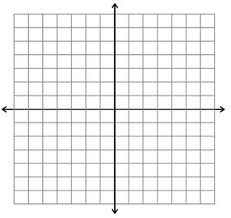
\includegraphics[scale=1.25]{images/plane}
\end{figure}
\vspace{1in}
\end{example}

\newpage

\begin{example}
Graph: $y > \dfrac{-3}{4}x$
\begin{figure}[h]
\hfill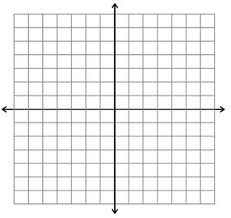
\includegraphics[scale=1.25]{images/plane}
\end{figure}
\vspace{1in}
\end{example}

\begin{example}
Graph: $x \le -2$
\begin{figure}[h]
\hfill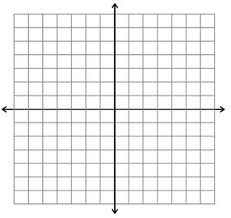
\includegraphics[scale=1.25]{images/plane}
\end{figure}
\vspace{1in}
\end{example}

\newpage

\begin{mdframed}
\textbf{Graphing Systems of Inequalities}

Systems of linear inequalities have a \emph{solution set} that is a portion of the plane, not just a point. To find this solution set, graph each of the inequalities individually and look for the overlap (intersection) of their solutions.
\end{mdframed}
\vspace{.2in}

\begin{example}
Graph the solution set of the following system:
\begin{align*}[left=\empheqlbrace]
x-3y&<6\\
 2x+3y&\ge -6
 \end{align*}
\begin{figure}[h]
\hfill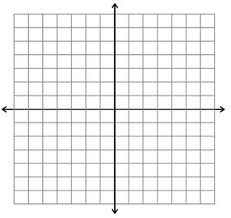
\includegraphics[scale=1.25]{images/plane}
\end{figure}
\vspace{1in}
\end{example}

\newpage

\begin{example}
Graph the solution set of the following system:
\begin{align*}[left=\empheqlbrace]
x+y&<2\\
-2\le x &< 1\\
 y &> -3
 \end{align*}
\begin{figure}[h]
\hfill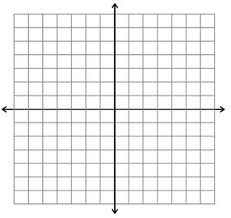
\includegraphics[scale=1.25]{images/plane}
\end{figure}
\vspace{1in}
\end{example}



\end{document}